\documentclass[border=8pt]{standalone}
\usepackage{amsmath,amssymb}
\usepackage{tikz}
\usetikzlibrary{arrows.meta,backgrounds}
\newcommand{\F}{\mathcal F}
\newcommand{\A}{\mathcal A}
\begin{document}
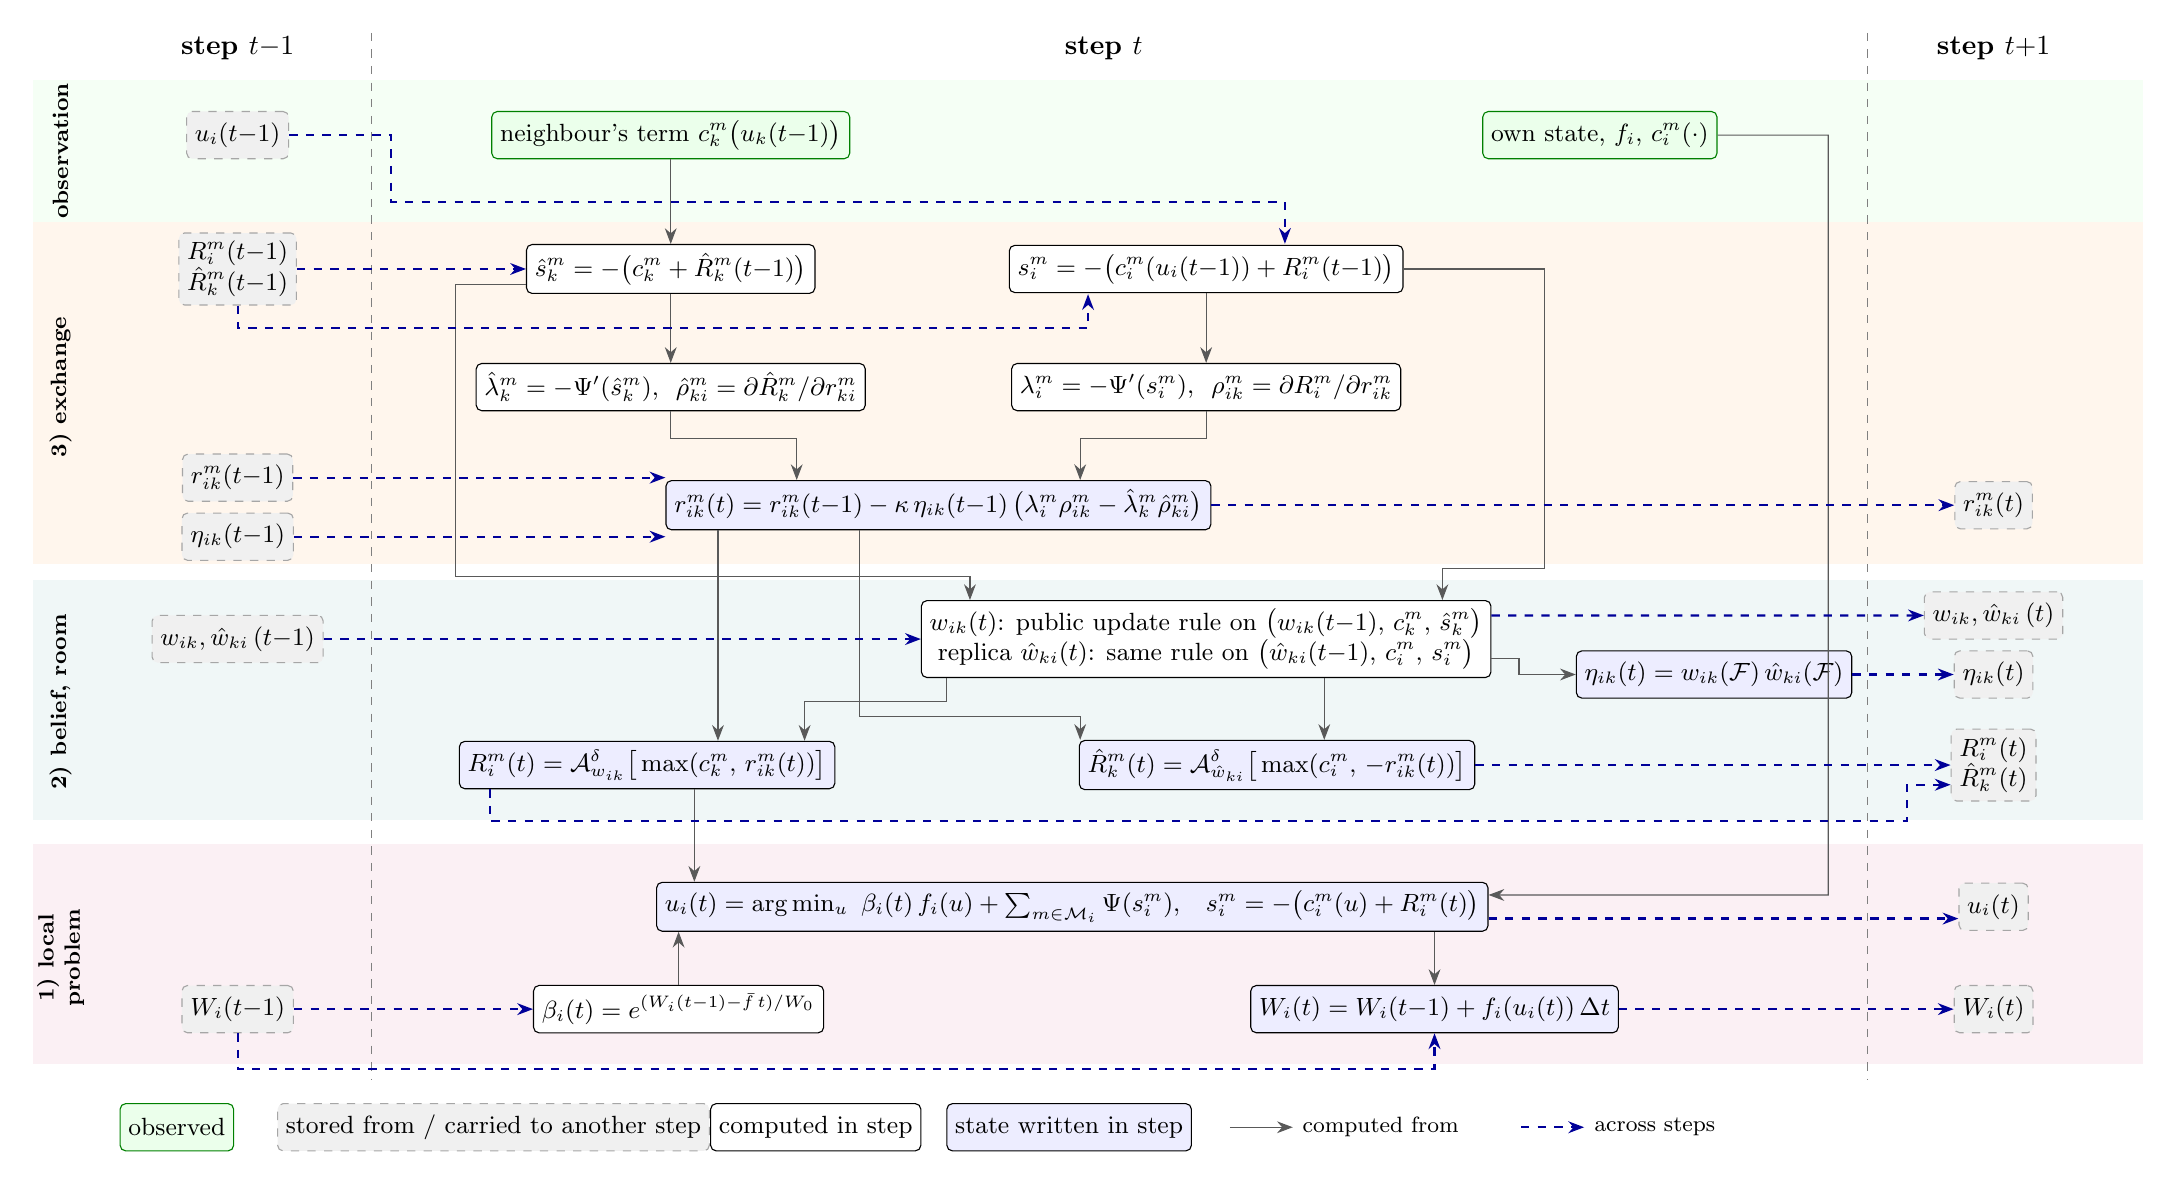
\begin{tikzpicture}[x=1cm,y=1cm,font=\small,>={Stealth[length=2mm]},
  obs/.style={draw=green!50!black,fill=green!8,rounded corners=2pt,inner sep=3pt,minimum height=6mm},
  sto/.style={draw=gray!70,fill=gray!12,dashed,rounded corners=2pt,inner sep=3pt,minimum height=6mm},
  cmp/.style={draw=black,fill=white,rounded corners=2pt,inner sep=3pt,minimum height=6mm},
  st/.style={cmp,fill=blue!7},
  e/.style={->,draw=black!65},
  carry/.style={->,draw=blue!60!black,dashed,thick}]
\def\yO{0}\def\yS{-1.7}\def\yL{-3.2}\def\yX{-4.7}\def\yB{-6.4}\def\yR{-8.0}\def\yQ{-9.8}\def\yW{-11.1}
\def\xa{0}\def\xb{22.3}
\begin{scope}[on background layer]
\fill[green!4] (-2.6,\yO+0.7) rectangle (24.2,\yO-1.1);
\fill[orange!7] (-2.6,\yS+0.6) rectangle (24.2,\yX-0.75);
\fill[teal!6] (-2.6,\yB+0.75) rectangle (24.2,\yR-0.7);
\fill[purple!6] (-2.6,\yQ+0.8) rectangle (24.2,\yW-0.7);
\draw[gray,dashed] (1.7,1.3)--(1.7,-12.0); \draw[gray,dashed] (20.7,1.3)--(20.7,-12.0);
\end{scope}
\node[font=\bfseries] at (\xa,1.1) {step $t{-}1$};
\node[font=\bfseries] at (11,1.1) {step $t$};
\node[font=\bfseries] at (\xb,1.1) {step $t{+}1$};
\node[rotate=90,font=\bfseries\footnotesize] at (-2.25,-0.2) {observation};
\node[rotate=90,font=\bfseries\footnotesize] at (-2.25,-3.2) {3) exchange};
\node[rotate=90,font=\bfseries\footnotesize] at (-2.25,-7.2) {2) belief, room};
\node[rotate=90,font=\bfseries\footnotesize,align=center] at (-2.25,-10.45) {1) local\\problem};

% stored
\node[sto] (uP) at (\xa,\yO) {$u_i(t{-}1)$};
\node[sto,align=center] (RP) at (\xa,\yS) {$R^m_i(t{-}1)$\\$\hat R^m_k(t{-}1)$};
\node[sto] (rP) at (\xa,\yX+0.35) {$r^m_{ik}(t{-}1)$};
\node[sto] (mP) at (\xa,\yX-0.4) {$\eta_{ik}(t{-}1)$};
\node[sto] (wP) at (\xa,\yB) {$w_{ik},\hat w_{ki}\,(t{-}1)$};
\node[sto] (WP) at (\xa,\yW) {$W_i(t{-}1)$};

% step t
\node[obs] (ck) at (5.5,\yO) {neighbour's term $c^m_k\big(u_k(t{-}1)\big)$};
\node[obs] (own) at (17.3,\yO) {own state, $f_i$, $c^m_i(\cdot)$};
\node[cmp] (sh) at (5.5,\yS) {$\hat s^m_k=-\big(c^m_k+\hat R^m_k(t{-}1)\big)$};
\node[cmp] (si) at (12.3,\yS) {$s^m_i=-\big(c^m_i(u_i(t{-}1))+R^m_i(t{-}1)\big)$};
\node[cmp] (lh) at (5.5,\yL) {$\hat\lambda^m_k=-\Psi'(\hat s^m_k)$,\ \ $\hat\rho^m_{ki}=\partial\hat R^m_k/\partial r^m_{ki}$};
\node[cmp] (li) at (12.3,\yL) {$\lambda^m_i=-\Psi'(s^m_i)$,\ \ $\rho^m_{ik}=\partial R^m_i/\partial r^m_{ik}$};
\node[st] (r) at (8.9,\yX) {$r^m_{ik}(t)=r^m_{ik}(t{-}1)-\kappa\,\eta_{ik}(t{-}1)\,\big(\lambda^m_i\rho^m_{ik}-\hat\lambda^m_k\hat\rho^m_{ki}\big)$};
\node[cmp,align=center] (bel) at (12.3,\yB) {$w_{ik}(t)$: public update rule on $\big(w_{ik}(t{-}1),\,c^m_k,\,\hat s^m_k\big)$\\ replica $\hat w_{ki}(t)$: same rule on $\big(\hat w_{ki}(t{-}1),\,c^m_i,\,s^m_i\big)$};
\node[st] (m) at (18.75,\yB-0.45) {$\eta_{ik}(t)=w_{ik}(\F)\,\hat w_{ki}(\F)$};
\node[st] (R) at (5.2,\yR) {$R^m_i(t)=\A^\delta_{w_{ik}}\big[\max(c^m_k,\,r^m_{ik}(t))\big]$};
\node[st] (Rh) at (13.2,\yR) {$\hat R^m_k(t)=\A^\delta_{\hat w_{ki}}\big[\max(c^m_i,\,-r^m_{ik}(t))\big]$};
\node[st] (qp) at (10.6,\yQ) {$u_i(t)=\arg\min_u\ \beta_i(t)\,f_i(u)+\sum_{m\in\mathcal M_i}\Psi(s^m_i)$,\quad $s^m_i=-\big(c^m_i(u)+R^m_i(t)\big)$};
\node[cmp] (bt) at (5.6,\yW) {$\beta_i(t)=e^{(W_i(t-1)-\bar f\,t)/W_0}$};
\node[st] (Wt) at (15.2,\yW) {$W_i(t)=W_i(t{-}1)+f_i(u_i(t))\,\Delta t$};

% carried
\node[sto] (rN) at (\xb,\yX) {$r^m_{ik}(t)$};
\node[sto] (wN) at (\xb,\yB+0.3) {$w_{ik},\hat w_{ki}\,(t)$};
\node[sto] (mN) at (\xb,\yB-0.45) {$\eta_{ik}(t)$};
\node[sto,align=center] (RN) at (\xb,\yR) {$R^m_i(t)$\\$\hat R^m_k(t)$};
\node[sto] (uN) at (\xb,\yQ) {$u_i(t)$};
\node[sto] (WN) at (\xb,\yW) {$W_i(t)$};

% within step t
\draw[e] (ck)--(sh); \draw[e] (sh)--(lh); \draw[e] (si)--(li);
\draw[e] (lh.south)--++(0,-0.35)-|([xshift=-18mm]r.north); \draw[e] (li.south)--++(0,-0.35)-|([xshift=18mm]r.north);
\draw[e] ([yshift=-2mm]sh.west)--++(-0.9,0)|-(6,-5.6)-|([xshift=-30mm]bel.north);
\draw[e] (si.east)-|(16.6,-5.5)-|([xshift=30mm]bel.north);
\draw[e] ([yshift=-2.5mm]bel.east)--++(0.35,0)|-(m.west);
\draw[e] ([xshift=-33mm]bel.south)--++(0,-0.3)-|([xshift=20mm]R.north);
\draw[e] ([xshift=15mm]bel.south)--([xshift=15mm]bel.south |- Rh.north);
\draw[e] ([xshift=-28mm]r.south)--([xshift=-28mm]r.south |- R.north);
\draw[e] ([xshift=-10mm]r.south)--([xshift=-10mm]r.south |- 0,-7.38)-|([xshift=-25mm]Rh.north);
\draw[e] ([xshift=6mm]R.south)--([xshift=6mm]R.south |- qp.north);
\draw[e] (own.east)-|(20.2,-9.65)--([yshift=1.5mm]qp.east);
\draw[e] (bt.north)--(bt.north |- qp.south);
\draw[e] ([xshift=46mm]qp.south)--([xshift=46mm]qp.south |- Wt.north);

% from t-1
\draw[carry] (uP.east)--(1.95,\yO)|-(13.3,-0.85)--(13.3,-1.38);
\draw[carry] (RP.east)--(sh.west);
\draw[carry] (RP.south)|-(10.8,-2.45)--(10.8,-2.02);
\draw[carry] (rP.east)--(rP.east -| r.west);
\draw[carry] (mP.east)--(mP.east -| r.west);
\draw[carry] (wP.east)--(wP.east -| bel.west);
\draw[carry] (WP.east)--(bt.west);
\draw[carry] (WP.south)--++(0,-0.45)-|(Wt.south);

% to t+1
\draw[carry] (r.east)--(rN.west);
\draw[carry] ([yshift=3mm]bel.east)--(wN.west);
\draw[carry] (m.east)--(mN.west);
\draw[carry] (Rh.east)--(RN.west);
\draw[carry] ([xshift=-20mm]R.south)--++(0,-0.4)-|(21.2,-8.25)--(RN.west |- 0,-8.25);
\draw[carry] ([yshift=-1.5mm]qp.east)--([yshift=-1.5mm]qp.east -| uN.west);
\draw[carry] (Wt.east)--(WN.west);

% legend
\node[obs,anchor=west] (L1) at (-1.5,-12.6) {observed};
\node[sto,anchor=west] (L2) at (0.5,-12.6) {stored from / carried to another step};
\node[cmp,anchor=west] (L3) at (6.0,-12.6) {computed in step};
\node[st,anchor=west] (L4) at (9.0,-12.6) {state written in step};
\draw[e] (12.6,-12.6)--(13.4,-12.6) node[right,font=\footnotesize] {computed from};
\draw[carry] (16.3,-12.6)--(17.1,-12.6) node[right,font=\footnotesize] {across steps};
\end{tikzpicture}
\end{document}
